%#BIBTEX bibtex Si$_3$N$_4$
\documentclass[twocolumn,amsmath,amssymb,a4paper,prb,superscriptaddress,floatfix]{revtex4-1}
\usepackage[dvipdfmx]{graphicx}
\usepackage{natbib}
\usepackage{multirow}
\usepackage{amsmath}
\usepackage{bm}
\usepackage{mathrsfs}
\usepackage{url}
\usepackage{color}
\usepackage{ulem}
\begin{document}

\title{First-principles calculation of the lattice thermal
conductivities of $\alpha$-, $\beta$-, and $\gamma$-Si$_3$N$_4$}

\author{Kazuyoshi Tatsumi} \email{k-tatsumi@imass.nagoya-u.ac.jp}
\affiliation{Advanced Measurement Technology Center, Institute of
Materials and Systems for Sustainability, Nagoya University, Chikusa,
Nagoya 464-8603, Japan}
\affiliation{Center for Elements Strategy
Initiative for Structural Materials, Kyoto University, Sakyo, Kyoto
606-8501, Japan}

\author{Atsushi Togo}
\affiliation{Center for Elements Strategy Initiative for Structural
Materials, Kyoto University, Sakyo, Kyoto 606-8501, Japan}

\author{Isao Tanaka}
\affiliation{Center for Elements Strategy Initiative for Structural
Materials, Kyoto University, Sakyo, Kyoto 606-8501, Japan}
\affiliation{Department of Materials Science and
Engineering, Kyoto University, Sakyo, Kyoto 606-8501, Japan}
\affiliation{Nanostructures Research Laboratory, Japan Fine Ceramics
Center, Atsuta, Nagoya 456-8587, Japan}

\begin{abstract}
Lattice thermal conductivities of $\alpha$-, $\beta$- and $\gamma$-Si$_3$N$_4$
single crystals are investigated from {\it ab-initio} anharmonic lattice
dynamics, within the single-mode relaxation-time approximation of the
linearized phonon Boltzmann transport equation. At 300 K, the lattice thermal
conductivity of $\beta$-Si$_3$N$_4$ is calculated as $\kappa_{xx}=73$ and
$\kappa_{zz}=198$ (in units of Wm$^{-1}$K$^{-1}$), that is consistent with the
reported experimental values of 69 and 180, respectively. For
$\alpha$-Si$_3$N$_4$, $\kappa_{xx}=69$ and $\kappa_{zz}=99$ are obtained.  The
difference of anisotropy between $\alpha$-Si$_3$N$_4$ and $\beta$-Si$_3$N$_4$
is originated from their characteristic difference in the phonon band
structures, originated from the difference in the crystal structures, {\it i.e.}, the
different stacking manners of equivalent basal layer structures.
In $\alpha$-Si$_3$N$_4$, acoustic-mode phonons below 6 THz are the
main heat carriers. In $\beta$-Si$_3$N$_4$, the phonon modes up to 12 THz
contribute to the lattice thermal conductivity. In $\gamma$-Si$_3$N$_4$,
$\kappa=81$ is obtained. The distribution of phonon mode contributions to
lattice thermal conductivity with respect to phonon frequency is found to
closely resemble $\kappa_{xx}$ of $\beta$-Si$_3$N$_4$ although the phonon
lifetimes of $\gamma$-Si$_3$N$_4$ are twice shorter than those of
$\beta$-Si$_3$N$_4$.
\end{abstract}

\maketitle

\section{Introduction}
Several nitride insulators are known to exhibit high thermal conductivities and
are important for heat transfer materials at elevated temperatures. For
example, Slack {\it et al.}~\cite{slack} reported that wurtzite-type AlN has
thermal conductivity of $\gg$  100 Wm$^{-1}$K$^{-1}$. \textcolor{blue}{Si$_3$N$_4$ has become
another promising thermal conductive insulator as its thermal conductivity has
been improved up to 177 Wm$^{-1}$K$^{-1}$ by using the advanced ceramic
technologies related to the densification and microstructure
control.~\cite{zhou,hirao-rev,watari,hirosaki}} Since the Si$_3$N$_4$ ceramics also
exhibit high mechanical strength at elevated temperatures, they are
regarded as ideal materials for the use in various applications, such as
engine components, gas turbines, and heat sink substrates of power
semiconductor devices.

At atmospheric pressure, Si$_3$N$_4$ exists in one of two phases, $\alpha$ and
$\beta$, which are generally considered as low- and high-temperature phases,
respectively.~\cite{zhou,hirosaki,riley} \textcolor {blue}{Their crystal structures belong to the
	space groups of P31c and P6$_3$/m, respectively.~\cite{yashima,boulay} These structures have 
different stacking orders of equivalent basal layer structures originated by SiN$_4$
tetrahedra.~\cite{hampshire} In Fig.\ref{fig:Fig1_cryst}  these layer structures are depicted from
the principal direction, as A, B, C, and D in the $\alpha$ phase and A and B in
the $\beta$ phase. The stacking manners in $\alpha$- and $\beta$-Si$_3$N$_4$ are
thus as ABCDABCD.. and ABAB.., respectively. 
The $\alpha$ phase has additional two layer structures of C and D, which are related to the A and B by
the $c$ glide operation.~\cite{hampshire} Along this direction the lattice constant of the $\alpha$ phase is
approximately two times longer than that of the $\beta$ phase.}
\begin{figure}[ht]
 \begin{center}
  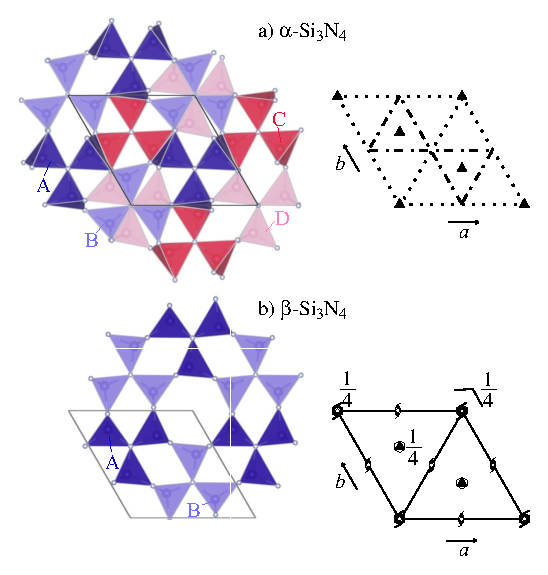
\includegraphics[width=0.90\linewidth]{Fig1_crystal_str2.eps} \caption{(color
  online) Crystal structures of $\alpha$- and $\beta$-Si$_3$N$_4$. Stacking of
  SiN$_4$ tetrahedron layers are shown in left. (a) ABCDABCD.. for
  $\alpha$-Si$_3$N$_4$. (b) ABAB.. for $\beta$-Si$_3$N$_4$.  Space group
  diagrams~\cite{inttableA} in P31c ($\alpha$-Si$_3$N$_4$) and P6$_3$/m ($\beta$-Si$_3$N$_4$)
  are shown in right.}
  \label{fig:Fig1_cryst} 
 \end{center}
\end{figure}

\textcolor{red}{The reported values~\cite{zhou,hirao-rev,watari,hirosaki,hirai}
of the thermal conductivity of the Si$_3$N$_4$ polymophs were measured on
pollycrystalline bulk samples. These values were significantly affected by
the contained lattice defects, impurities, shapes and orientations of the
constituent crystal grains;~\cite{hirosaki-md} the thermal conductivity intrinsic to a
defect-free single crystal has not been established. As
an experimental approach to the intrinsic thermal conductivity,} Li {\it et
al.}~\cite{li} applied high-resolution thermoreflectance microscopy to single
$\beta$-Si$_3$N$_4$ grains in a ceramic sample. The analyzed thermal
conductivities were 69 and 180 Wm$^{-1}$K$^{-1}$ along the $a$ and $c$ axes,
respectively. \textcolor{red}{These thermal conductivities correspond to the
$xx$ and $zz$  elements of the lattice thermal conductivity tensor
$\boldsymbol{\kappa}$.} We consider the anisotropy of
$\kappa_{zz}/\kappa_{xx}\sim 3$ is relatively large.  Theoretically, Hirosaki
{\it et al.}~\cite{hirosaki-md} estimated $\boldsymbol{\kappa}$ by
applying the Green-Kubo formulation to the molecular dynamics (MD) method with
the interatomic potentials proposed by Vashishta {\it et al.}~\cite{vashishta}. 
They calculated $\kappa$$_{xx}$ and $\kappa$$_{zz}$ of
$\alpha$-Si$_3$N$_4$ as 105 and 225 Wm$^{-1}$K$^{-1}$, and those of
$\beta$-Si$_3$N$_4$ as 170 and 450 Wm$^{-1}$K$^{-1}$, respectively.
The ratio $\kappa_{zz}/\kappa_{xx}$ in $\beta$-Si$_3$N$_4$ agreed well with the
experimental one: The $\kappa_{ii}$
values overestimated the experimental ones by more than two times. 

On many polymorphs of the wurtzite and zincblende structures, the lattice
thermal conductivities were recently calculated based on a first principles
calculation and Boltzman transport theory.~\cite{phono3py}  These crystal
structures
have different stacking orders of the densest atom planes as ABAB.. and
ABCABC...  The different stacking orders merely altered the lattice thermal
conductivities.~\cite{phono3py} The phonon linewidth distribution and phonon
density of states were similar between the structures as well.~\cite{phono3py}
On the other hand, the previous MD results on $\alpha$- and
$\beta$-Si$_3$N$_4$ presented that the different stacking orders in these
phases altered $\boldsymbol{\kappa}$ largely. This
has not been explained through the phonon properties.
It is interesting to investigate it using the same approach as in
Ref.\onlinecite{phono3py}.

In addition to the $\alpha$ and $\beta$ phases, a cubic spinel phase
($\gamma$-Si$_3$N$_4$) is known to form upon compression and in-situ
heating.~\cite{zerr,zhang} The reported transition pressures were scattered
from 10 to 36 GPa depending on the experimental conditions.~\cite{xu}  The
$\gamma$ phase is experimentally quenched to atmospheric pressure at room
temperature.  Its thermal conductivity has not been experimentally reported; it
has been estimated only by the Slack model.~\cite{morelli} 

The present study aims to qualitatively understand the lattice thermal
conductivity tensors among the three Si$_3$N$_4$ phases by means of the first
principles approach.  \textcolor{blue}{We calculate $\boldsymbol{\kappa}$ of
the $\gamma$ phase as well, for systematic understanding of the lattice
thermal conductivity in the Si$_3$N$_4$ system.  After the methodology
section, we examine the validity of the present results first.  Our
calculated thermal properties are compared with the available experimental
and theoretical references.  Then we investigate the characteristics in the
calculated $\boldsymbol{\kappa}$ in detail on the basis of the phonon band
structures and phonon linewidths.}

\section{Computational procedures}

\subsection{Lattice thermal conductivity calculation}

The lattice thermal conductivities were calculated by solving the linearized
Boltzmann transport equation (LBTE) within the single-mode relaxation time
approximation (single-mode RTA).  We also tried the direct-solution of
LBTE~\cite{chaput-direct} and leave its calculated $\boldsymbol{\kappa}$ values
in the following section. The differences between the
$\boldsymbol{\kappa}$ calculated by the single-mode RTA and the direct solution
were found minor for our discussion. Therefore we limited our research to use
the single-mode RTA to take advantage of its intuitive closed form of
$\boldsymbol{\kappa}$.

In the following sections, we denote a phonon mode by $\lambda=(\mathbf{q},p)$
with the set of the phonon wave vector $\mathbf{q}$ and band index $p$ and $-\lambda \equiv (-\mathbf{q},p)$. The
relaxation time due to phonon-phonon scattering was obtained as reciprocal of
linewidth, $\tau_{\lambda,\text{ph-ph}}=(2\Gamma_\lambda)^{-1}$, where the
linewidth that we employed in this study is as follows:
\begin{align}
 \label{eq:linewidth}
 &\Gamma_\lambda = \frac{18\pi}{\hbar^2}
  \sum_{\lambda' \lambda''}
  \bigl|\Phi_{-\lambda\lambda'\lambda''}\bigl|^2 \times \nonumber \\ 
 &\left\{ (n_{\lambda'} + n_{\lambda''}+1) 
   \delta(\omega_\lambda-\omega_{\lambda'}-\omega_{\lambda''}) \right.
   + \nonumber \\ 
 &\;\;(n_{\lambda'}-n_{\lambda''})
  \left[\delta(\omega_\lambda +\omega_{\lambda'}-\omega_{\lambda''})
 \right. 
 \left. -\left. \delta(\omega_\lambda - \omega_{\lambda'}+\omega_{\lambda''})
 \right]\right\}.
\end{align}
Here $\omega_\lambda$ is the harmonic phonon frequency of the phonon mode
$\lambda$, $n_\lambda=[\exp(\hbar\omega_\lambda/\mathrm{k_B}T)-1]^{-1}$ is
the Bose-Einstein distribution at temperature $T$, and
$\Phi_{\lambda\lambda'\lambda''}$ denotes the three-phonon-scattering strength.
$\Phi_{\lambda\lambda'\lambda''}$ was obtained by usual coordinate
transformation of third-order force constants from direct space to phonon
space.~\cite{phono3py} The second- and third-order real-space force constants
were obtained from the {\it ab-initio} calculation, whose details are written in the
next section.

In order to compare the more realistic results of the calculated $\boldsymbol{\kappa}$ with the
experimental data, the isotopic scattering effect due to the natural isotope
distribution was taken into account according to the second-order perturbation
theory.~\cite{tamura} With the relaxation times of the phonon-phonon scattering
and isotopic scattering, $\tau_{\lambda,\text{ph-ph}}$ and
$\tau_{\lambda,\text{iso}}$, the total relaxation time for a phonon mode was
assumed to be $1/\tau_{\lambda} = 1/\tau_{\lambda,\text{ph-ph}} +
1/\tau_{\lambda,\text{iso}}$, according to Matthiessen's rule.

The available experimental thermal conductivity data of the Si$_3$N$_4$ system
have been measured on the polycrystalline samples and not measured from any
single crystals. In order to consider the effect of various lattice defects in
the polycrystalline samples, such as grain boundaries, impurities, and
vacancies, we crudely took them into account by a relaxation time
$\tau_{\lambda,\text{bs}}=L/|\mathbf{v}_\lambda|$ of a phonon boundary
scattering model, where $\mathbf{v}_\lambda =
\nabla_{\mathbf{q}}\omega_\lambda$ is the group velocity and $L$ a
parameter regarding to the boundary mean free path. We consider
$\tau_{\lambda,\text{bs}}$ as a variable parameter and included it to
$\boldsymbol{\kappa}$ according to Matthiessen's rule.

The closed form of $\boldsymbol{\kappa}$ within RTA was obtained via
\begin{align}
 \label{eq:kappa}
 \boldsymbol{\kappa}(T) = \frac{1}{N_\mathbf{q}\Omega} \sum_\lambda
 \tau_\lambda(T) \mathbf{v}_\lambda \otimes \mathbf{v}_\lambda c_\lambda(T),
\end{align}
where $N_\mathbf{q}$ is the number of
$\mathbf{q}$-points, $\Omega$ is the unit cell volume, and $c_\lambda$
is the mode heat capacity. To analyze $\boldsymbol{\kappa}$ in detail, we calculate
the cumulative thermal conductivity:
\begin{align}
 \label{eq:cum-kappa}
 \boldsymbol{\kappa}^\text{c}(\omega) = \frac{1}{N_\mathbf{q}\Omega}
 \int_0^\omega \sum_\lambda
 \tau_\lambda(T) \mathbf{v}_\lambda \otimes \mathbf{v}_\lambda
 c_\lambda(T) \delta(\omega'-\omega)d\omega',
\end{align}
and its derivative $\frac{\partial
\boldsymbol{\kappa}^\text{c}(\omega)}{\partial \omega}$ to see the phonon mode
contributions to $\boldsymbol{\kappa}$.

The lattice thermal conductivities were calculated with the phonon-phonon interaction calculation code
PHONO3PY~\cite{phono3py}, while the harmonic phonon states were analyzed with
the phonon calculation code PHONOPY~\cite{phonopy}.

\subsection{Computational details}

The force constants were calculated using the first-principles projector
augmented wave method~\cite{paw} (VASP code~\cite{vasp-1996,vasp-1995,
vasp-1999}). The generalized gradient approximation (GGA) parameterized by
Perdew, Burke, and Ernzerhof~\cite{pbe} was used for the exchange correlation
potential. A plane wave energy cutoff of 500 eV was employed. The crystal
structures were optimized until the residual forces acting
on the constituent atoms were less than $10^{-6}$ eV/\AA. The structural
optimization was firstly performed for a temperature of 0 K and 0 GPa. Here the
temperature and pressure were considered only for the electronic system and the
zero point lattice vibration was not taken into account. The calculated lattice
parameters were $a=7.808$ \AA~ and $c=5.659$ \AA~ for the $\alpha$ phase,
$a=7.660$ \AA~ and $c=2.925$ \AA~ for the $\beta$ phase, and $a=7.787$ \AA~
for the $\gamma$ phase, which agree with the experimental
data~\cite{yashima,boulay,paszkowicz} within +0.7 \% errors. The lattice
volume optimized within the local density approximation
(LDA)~\cite{lda} for the exchange correlation potential was, for
$\beta$-Si$_3$N$_4$, 3 \% smaller than within GGA, which is a typical
volume contraction of LDA. The $\boldsymbol{\kappa}$ calculated within LDA was larger by 2.6 \% than within GGA. For
our discussion, this difference is enough small, therefore the impact of
choice of exchange correlation potential is considered to be minor in our
study.

\begin{table}[ht]
	\caption{\label{table:LTC} Calculated lattice thermal conductivities 
 of $\alpha$-, $\beta$-, and $\gamma$-Si$_3$N$_4$
 (WK$^{-1}$m$^{-1}$) at 300 K with respect to several combinations of
 supercell sizes.}
 \begin{ruledtabular}
  \begin{tabular}{ccccc}
   \multirow{2}{*}{Phase}
   & \multicolumn{2}{c}{Supercell (\# of atoms)} &
   \multicolumn{2}{c}{LTC} \\
   \cline{2-5}
   & $3^\text{rd}$ force constants & $2^\text{nd}$ force constants & $xx$ & $zz$ \\
   \hline
   \multirow{6}{*}{$\alpha$}
   & $1\times 1\times 1$ (28) & $1\times
   1\times 1$ (28) & \textcolor{blue}{37} &   \textcolor{blue}{57} \\ 
   & $1\times 1\times 2$ (56) & $1\times
   1\times 2$ (56) & \textcolor{blue}{41} &   \textcolor{blue}{79} \\ 
   & $1\times 1\times 1$ (28) & $2\times
   2\times 2$ (224) & \textcolor{blue}{55} &   \textcolor{blue}{81} \\ 
   & $1\times 1\times 2$ (56) & $2\times
   2\times 2$ (224) & \textcolor{blue}{67} &   \textcolor{blue}{95} \\ 
   & $1\times 1\times 2$ (56) & $2\times
   2\times 3$ (336) & \textcolor{blue}{68} &  \textcolor{blue}{97} \\ 
   & $1\times 1\times 2$ (56) & $3\times
   3\times 4$ (1008) & \textcolor{blue}{68} &  \textcolor{blue}{100} \\ 
   \hline
   \multirow{5}{*}{$\beta$}
   & $1\times 1\times 2$ (28) & $1\times
   1\times 2$ (28) & \textcolor{blue}{44} & \textcolor{blue}{173} \\ 
   & $1\times 1\times 2$ (28) & $2\times
   2\times 4$ (224) & \textcolor{blue}{76} &  \textcolor{blue}{208} \\ 
   & $1\times 1\times 3$ (42) & $2\times
   2\times 4$ (224) & \textcolor{blue}{71} & \textcolor{blue}{194} \\ 
   & $1\times 1\times 3$ (42) & $2\times
   2\times 5$ (280) & \textcolor{blue}{72} & \textcolor{blue}{196} \\ 
   & $1\times 1\times 3$ (42) & $3\times
   3\times 8$ (1008) & \textcolor{blue}{73} & \textcolor{blue}{199} \\ 
   \hline
   \multirow{3}{*}{$\gamma$}
   & $1\times 1\times 1$ (56) & $1\times
   1\times 1$ (56) & \multicolumn{2}{c}{\textcolor{blue}{72}} \\ 
   & $1\times 1\times 1$ (56) & $2\times
   2\times 2$ (448) & \multicolumn{2}{c}{\textcolor{blue}{77}} \\ 
   & $1\times 1\times 1$ (56) & $3\times
   3\times 3$ (56) & \multicolumn{2}{c}{\textcolor{blue}{79}} \\ 
  \end{tabular}
 \end{ruledtabular}
\end{table}

Supercell and finite difference approaches were used to calculate the
force constants.~\cite{wei-supercell} The supercells were $1\times 1\times2$, $1\times
1\times3$, and $1\times 1\times1$ supercells of the conventional unit cells for
the calculation of the third-order force constants in $\alpha$, $\beta$, and
$\gamma$-Si$_3$N$_4$, respectively; $3\times 3\times4$, $3\times
3\times8$ and $2\times 2\times2$ for the second-order force constants.  The length of the
induced atomic displacement was set to 0.03 \AA.  Table \ref{table:LTC} shows
the $\boldsymbol{\kappa}$  calculated with several different sets of the supercells,
indicating that our calculated $\boldsymbol{\kappa}$ is reasonably converging with respect to
the size of the supercells. 

\textcolor{blue}{Non-analytical term correction~\cite{wang} was applied to the
second-order force  constants to take into account the long range Coulomb forces present in
ionic crystals. For the correction, static dielectric constants and Born effective charges were calculated by
using the density functional perturbation theory (DFPT) as implemented in the
VASP code~\cite{vasp-lepsiron,lepsiron}}.

Uniform $\mathbf{k}$-point sampling meshes of $4\times 4\times 2$,
$4\times 4\times 3$, and $3\times 3\times 3$ were used for the
third-order force constants of the $\alpha$, $\beta$, and $\gamma$ phases. For the
$\alpha$ and $\beta$ phases the center of the $a^*b^*$ plane was sampled
while the center on the $c^*$-axis was not. For the
$\gamma$ phase, non-$\Gamma$ center mesh was used. For the second-order
force constants, the $\Gamma$-point was only sampled for the $\alpha$ and $\beta$
phase and the only one $\mathbf{k}=(0.5, 0.5, 0.5)$ point was
sampled for the $\gamma$ phase. The $\mathbf{q}$-point
sampling meshes of $10\times 10\times 14$, $10\times 10\times 26$, and
$12\times 12\times 12$ were used to calculate $\boldsymbol{\kappa}$ in Eq.~(\ref{eq:kappa})
for the $\alpha$, $\beta$, and $\gamma$ phases.

\textcolor {blue}{We examined the effect of thermal expansion on
	$\boldsymbol{\kappa}$. We calculated the $\boldsymbol{\kappa}$ with the crystal structures
optimized for several finite temperatures within the quasi-harmonic
approximation (QHA)~\cite{dove-p76}.  
These $\boldsymbol{\kappa}$ were different from theose for the
corresponding etemperatures, calculated with the structure optimized for 0 K and 0 GPa. We
consider these differences as the effect of thermal expansion.
For $\beta$-Si$_3$N$_4$ and temperatures of 300, 600, 900,
1200, and 1500 K, the differences in $\boldsymbol{\kappa}$ 
were found less than 1 \%, similar to the case of Si and
Ge~\cite{ward-ltc}. For the present study, these differences are negligible
and we adopt the $\boldsymbol{\kappa}$ calculated with the structure
optimized for 0 K and 0 GPa.}


We calculated the volumetric thermal expansion coefficients and compared them
with the reported experimental values so as to check the validity of the
present thermal conductivity calculation, because the thermal expansion is
originated from the anharmonicity of the interatomic potential as well as
$\boldsymbol{\kappa}$. The calculated values of the $\alpha$ and $\beta$ phases
are 4.31$\times 10^{-6}$ and 4.19$\times 10^{-6}$ K$^{-1}$ for 300 K , while
the experimental values~\cite{minikayev-alpha} were 3.75$\times 10^{-6}$ and
3.55$\times 10^{-6}$ K$^{-1}$). The present calculation reproduced the
experimental tendency where the $\alpha$ phase has a slightly larger thermal
expansion coefficient than the $\beta$ phase, supporting that the present
calculations enable us to qualitatively compare the calculated
$\boldsymbol{\kappa}$ among the Si$_3$N$_4$ phases.

In order to compare the microscopic phonon properties among the three phases at
the same conditions, those results calculated at 0 GPa are shown and discussed.
For the $\gamma$ phase, this means that we assume the condition of a virtually
quenched $\gamma$ phase at 0 GPa from the high pressure. To examine the
analytical continuity of the properties with respect to pressures, we
calculated $\boldsymbol{\kappa}$ of the $\gamma$ phase at 10, 20, and 40 GPa as
shown in Fig.~\ref{fig:S1}. The phenomenological behaviour of linear dependence
of $\boldsymbol{\kappa}$ with respect to pressure was reproduced as similar to
Ref.~\onlinecite{andersson-pressure}. The slope was 2.89
Wm$^{-1}$K$^{-1}$GPa$^{-1}$ for the $\gamma$ phase.  By this dependence, we
consider that the microscopic values are also varied smoothly with the pressure
and those at 0 GPa are valuable to compare with the $\alpha$ and $\beta$
phases.

\subsection{Direct solution of LBTE}

The merit to employ the single-mode RTA for thermal conductivity calculation is
the closed form, by which we can intuitively understand the qualitative
character of $\boldsymbol{\kappa}$ in terms of the relaxation time and group velocity. The
microscopic understanding of the full solution of LBTE is still under the
development~\cite{cepellotti-relaxons} and the microscopic picture based on
collective phonons~\cite{hardy-collective} will require more complicated
investigation although it is known that the single-mode RTA solution of LBTE
often underestimates the full solution.~\cite{mukhopadhyay-ltc,ward-ltc}

On the $\boldsymbol{\kappa}$ of the $\alpha$ and $\beta$ phases, we adopted a
direct solution of LBTE~\cite{chaput-direct}, which is one of the methods of
LBTE full solutions. Their $\kappa_{xx}$ and $\kappa_{zz}$ without the isotope
effect were 69 and 102 Wm$^{-1}$K$^{-1}$ for  the $\alpha$ phase and 76 and 238
Wm$^{-1}$K$^{-1}$ for the $\beta$ phase, respectively, while the corresponding
single-mode RTA values were 70 and 102 Wm$^{-1}$K$^{-1}$ for the $\alpha$ phase
and 76 and 210 Wm$^{-1}$K$^{-1}$ for the $\beta$ phase. The $\kappa_{zz}$ of
the direct solution in the $\beta$ phase was 13 \% larger than that of the
single-mode RTA solution. Since the differences in $\boldsymbol{\kappa}$
between the LBTE solutions are not significant, we expect the physics on those
lattice thermal conductivities is well understood within RTA in the current
level of our interest.  \textcolor {red} {Therefore, we discuss the lattice
thermal conductivities using  the results of the single-mode RTA solution.}

\section{Results and discussion}

\subsection{Lattice thermal conductivities}

\begin{table}[ht]
 \caption{\label{table:LTC-exp} Calculated thermal conductivities of
 $\alpha$-Si$_3$N$_4$ (trigonal), $\beta$-Si$_3$N$_4$ (trigonal), and
 $\gamma$-Si$_3$N$_4$ (cubic) at 300
 K, compared with the experimental data. Theoretical bulk moduli $B$ in
 units of GPa, calculated by the authors by using the present band
 method, are presented in the fourth column.}
% \begin{ruledtabular}
%  \begin{tabular}{cccccccccc}
%   & \multicolumn{3}{c}{This work} & \multicolumn{3}{c}{\textcolor{red}{Ref. Theo.}}
%   & \multicolumn{3}{c}{Ref. Expt.} \\
%   \cline{2-10}
%   & $\kappa_{xx}$ & $\kappa_{zz}$ & $B$ & $\kappa$ & $\kappa_{xx}$ & $\kappa_{zz}$ & $\kappa$ & $\kappa_{xx}$ & $\kappa_{zz}$ \\
%   \hline
%   $\alpha$-Si$_3$N$_4$ & \textcolor{blue}{68} & \textcolor{blue}{100} & 224 & 70\footnotemark[1] & 105\footnotemark[2] & 225\footnotemark[2] & 59\footnotemark[4] & - & -  \\
%   $\beta$-Si$_3$N$_4$ & \textcolor{blue}{73} & \textcolor{blue}{199} & 237 & 250\footnotemark[1] & 170\footnotemark[2] & 450\footnotemark[2] & 122\footnotemark[5] & 69\footnotemark[6] & 180\footnotemark[6] \\
%   $\gamma$-Si$_3$N$_4$ & \textcolor{blue}{77} & - & 296 & 80\footnotemark[1] & - & - & - & - & - 
%   \footnotetext[1]{Ref.~\onlinecite{morelli}, Slack model.}
%   \footnotetext[2]{Ref.~\onlinecite{hirosaki-md}, molecular dynamics (Green-Kubo).}
%   \footnotetext[4]{Ref.~\onlinecite{hirai}, thin film.}
%   \footnotetext[5]{Ref.~\onlinecite{hirosaki}, poly-crystals.}
%   \footnotetext[6]{Ref.~\onlinecite{li}, single crystalline grains of poly-crystals.}
%  \end{tabular}
% \end{ruledtabular}
%\end{table}

\begin{ruledtabular}
 \begin{tabular}{ccccccccc}
   & \multicolumn{3}{c}{This work} & \multicolumn{3}{c}{\textcolor{red}{Ref. Theo.}}
   & \multicolumn{2}{c}{Ref. Expt.} \\
   \cline{2-9}
   & $\kappa_{xx}$ & $\kappa_{zz}$ & $B$ & $\kappa$ & $\kappa_{xx}$ & $\kappa_{zz}$ & $\kappa_{xx}$ & $\kappa_{zz}$ \\
   \hline
   $\alpha$-Si$_3$N$_4$ & \textcolor{blue}{68} & \textcolor{blue}{100} & 224 & 70\footnotemark[1] & 105\footnotemark[2] & 225\footnotemark[2] & - & -  \\
   $\beta$-Si$_3$N$_4$ & \textcolor{blue}{73} & \textcolor{blue}{199} & 237 & 250\footnotemark[1] & 170\footnotemark[2] & 450\footnotemark[2] & 69\footnotemark[3] & 180\footnotemark[3] \\
   $\gamma$-Si$_3$N$_4$ & \textcolor{blue}{77} & - & 296 & 80\footnotemark[1] & - & - & - & - 
   \footnotetext[1]{Ref.~\onlinecite{morelli}, Slack model.}
   \footnotetext[2]{Ref.~\onlinecite{hirosaki-md}, molecular dynamics (Green-Kubo).}
   \footnotetext[3]{Ref.~\onlinecite{li}, single crystalline grains of poly-crystals.}
  \end{tabular}
 \end{ruledtabular}
\end{table}

Table \ref{table:LTC-exp} shows the present results of the
$\boldsymbol{\kappa}$ for 300 K.  $\beta$-Si$_3$N$_4$ has markedly more
anisotropic $\boldsymbol{\kappa}$ than $\alpha$-Si$_3$N$_4$.  The directional
averages $\sum_i \kappa_{ii}/3$  are 79, 115,  and 77 Wm$^{-1}$K$^{-1}$ for the
$\alpha$, $\beta$, and $\gamma$ phases, respectively.  The value of the
$\gamma$ phase is similar to that of the $\alpha$ phase, in spite of
comparatively large difference among the bulk moduli ($B$) that are also shown
in Table \ref{table:LTC-exp}.   

Table \ref{table:LTC-exp} also shows the previously reported
experimental~\cite{li} and theoretical~\cite{hirosaki-md} thermal
conductivities for the references.  Previously Morelli {\it et
al.}~\cite{morelli} employed the Slack model for estimating the lattice thermal
conductivities of the three phases. They are shown as $\kappa$ in Table
\ref{table:LTC-exp}. For the $\beta$ phase, our $\boldsymbol{\kappa}$ agrees
better with the experimental, than that of the molecular
calculation~\cite{hirosaki-md} does.  Also, our directional average $\sum_i
\kappa_{ii}/3$ is much closer to the experimental
average, than the $\kappa$ of the Slack model.

Fig.~\ref{fig:Fig1_338} shows the theoretical $\boldsymbol{\kappa}$ of the
$\alpha$ and $\beta$ phases as a function of $T$, together with the reference
experimental data~\cite{hirosaki,hirai}. The thermal conductivities for a
series of temperatures were only reported on the polycrystalline bulk samples
and measured by the laser flash method. 
These thermal conductivities (denoted as $\kappa_\mathrm{polycrystal}$) cannot be directly compared with the
calculated intrinsic $\boldsymbol{\kappa}$ because they 
largely depended on the microstructure of the samples: 
They were deviated from the simple directional averages of the
intrinsic $\kappa_{ii}$, depending on the shapes of the crystal
grains.  We treated this effect by using a parameter $0\le{w}\le{1}$ and
fitting the quantities of $w\kappa_{xx} + (1-w) \kappa_{zz}$ to the experimental
$\kappa_\mathrm{polycrystal}$ by the least squares method. We consider these as
theoretical $\kappa_\mathrm{polycrystal}$. 

\begin{figure}[ht]
 \begin{center}
  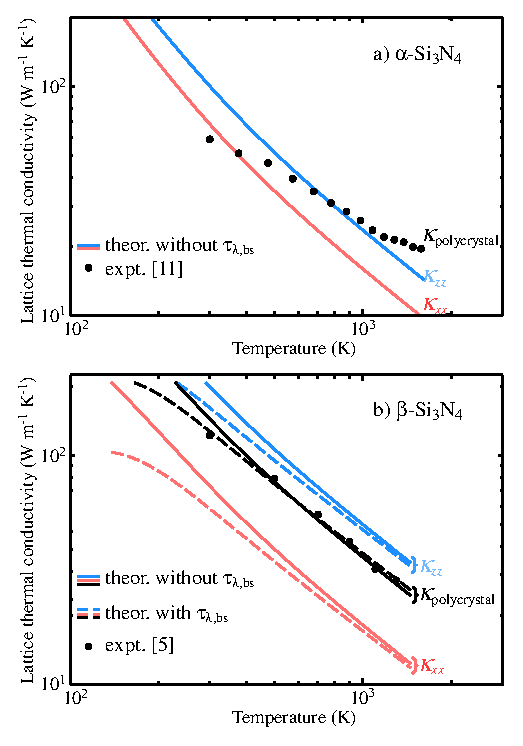
\includegraphics[width=0.90\linewidth]{Fig1_m1010.eps} \caption{(color
  online) Temperature dependence of thermal conductivities for $\alpha$- and
  $\beta$-Si$_3$N$_4$. For $\beta$-Si$_3$N$_4$, theoretical results with the
  boundary scattering effect are shown by broken lines. Theoretical
  $\kappa_\mathrm{polycrystal}$ 
  (see in text) for the $\beta$-Si$_3$N$_4$ sample are
  also shown to be compared with the experimental conductivities.}
  \label{fig:Fig1_338}
 \end{center}
\end{figure}

\textcolor {blue}{In Fig.~\ref{fig:Fig1_338}, the $\kappa_{ii}$ calculated
without $\tau_{\lambda,\text{bs}}$ are nearly proportional to $T^{-1}$ because
$n_\lambda$ in Eq.~(\ref{eq:linewidth}) can be reduced to
$\exp(-\hbar\omega_\lambda/\mathrm{k_B}T)$.} In Fig.~\ref{fig:Fig1_338}-a, the
experimental $\kappa_\mathrm{polycrystal}$ of a
chemically vapor-deposited $\alpha$-Si$_3$N$_4$ sample~\cite{hirai} is not
proportional to $T^{-1}$ and intersects the theoretical $\kappa_{ii}$.  Thus
no value of $w$ adjusts the theoretical conductivities to the experimental
data.  The full solution of LBTE would negligibly cure the disagreement.
Including the simple phonon lifetime of boundary scattering,
$\tau_{\lambda,\text{bs}}=L/|\mathbf{v}_\lambda|$, into the total phonon
lifetime according to Matthiessen's rule, could not explain the discrepancy as
well.  \textcolor {blue}{A $L$ value of 0.6 $\mu\text{m}$, which was much
smaller than the experimental grain size~\cite{hirai} of 10 $\mu\text{m}$,} decreased the
theoretical $\kappa$$_{ii}$ in the low temperature side toward
the experimental values, but severely underestimated in
the high temperature side.  At present, the reason for the discrepancy between
the theoretical and experimental behaviors is unclear.  Although the crystal
structure of the experimental sample was characterized as $\alpha$-Si$_3$N$_4$,
significant lattice defects existed in the as-deposited sample as pointed
out by Hirosaki {\it et al.}~\cite{hirosaki-md} and \textcolor{blue}{the simple
phonon boundary scattering model may fail to describe their effects on the
$\kappa_\mathrm{polycrystal}$.} 

The experimental $\kappa_\mathrm{polycrystal}$ of the $\beta$ phase are located
in-between the theoretical $\kappa$$_{xx}$ and  $\kappa$$_{zz}$, being nearly
proportional to $T^{-1}$. Simple directional averages of the theoretical
$\kappa_{ii}$ slightly underestimate these experimental values.  This is
understood from the fact that the microstructure was controlled to increase the
$\kappa_\mathrm{polycrystal}$, and the crystalline grains were selectively grown along
the $c$ axis of the most conductive direction.~\cite{hirosaki} The theoretical
$\kappa_\mathrm{polycrystal}$ were fit well with $w=\textcolor{blue}{0.44}$  to
the experimental.  For the effects of lattice
defects most of which were grain boundaries, we included
$\tau_{\lambda,\text{bs}}$ with $L = \textcolor{blue}{0.6}$ $\mu\text{m}$ to
further fit the theoretical curve ($w=\textcolor{blue}{0.33}$) to the
experimental data.  The $L$ value is \textcolor{blue}{slightly smaller than}
the average grain size~\cite{hirosaki} of 2 $\mu\text{m}$ in the experiment.
%The experimental $\kappa$$_{ii}$ are rather close to the theoretical
%$\kappa$$_{ii}$ calculated without $\tau_{\lambda,\text{bs}}$.  This is
%explained by the fact that the experimental $\kappa$$_{xx}$ and
%$\kappa$$_{zz}$ were deduced consistently through the grains of several
%different sizes. The effects of the phonon scattering at the grain boundaries
%were eliminated.~\cite{li}


\subsection{Dispersion curves}

Figure \ref{fig:Fig4_ver5_338} shows the phonon band diagrams of the three
Si$_3$N$_4$ phases. The entire band diagrams are almost identical to those
reported earlier~\cite{kuwabara,xu}. However, here we investigate the gradients
of the band dispersions, that is, the group
velocities projected on the high-symmetry paths. We especially focus on their
anisotropy in the $\alpha$ and $\beta$ phases. This was
not investigated by the previous works.

\begin{figure}[ht]
 \begin{center}
  \includegraphics[width=0.90\linewidth]{Fig4_ver5_338_resize2_woDOS.eps}
  \caption{(color online) Brillouin-zones (left) and calculated phonon band diagrams (right) for three Si$_3$N$_4$ phases.
  \label{fig:Fig4_ver5_338} }
 \end{center}
\end{figure}

%The acoustic branches in the $\alpha$ phase highlighted in red in
%Fig.~\ref{fig:Fig4_ver5_338}-a do not increase their frequencies much more than
%those along the other paths, $\Gamma$--K or $\Gamma$--M. The frequency maxima
%along the $\Gamma$--A path are around 7 THz, rather close to the maxima along
%the $\Gamma$--K and $\Gamma$--M paths (around 5 THz). The upper branches along
%the $\Gamma$--A path are also as flat as the upper branches along the
%$\Gamma$--K and $\Gamma$--M paths.  In contrast, in the band diagram of the
%$\beta$ phase (Fig.~\ref{fig:Fig4_ver5_338}-b), the acoustic phonon branches
%highlighted in red along the $\Gamma$--A path increase their frequencies almost
%linearly from the $\Gamma$-point to the A-point and reach around 10 THz, along
%which the group velocity component $v_{\lambda,z}$ maintains high values.
The $\omega_{\lambda}$ of the acoustic branches in the $\beta$ phase increase
much more from $\Gamma$ to A than from $\Gamma$ to K or M.  In the $\alpha$
phase, $\omega_{\lambda}$ increase similarly among the paths.
This difference is due to the different $\Gamma$-A path lengths.  The
$\beta$ phase has an approximately twice longer path than the $\alpha$ phase;
the lattice constant $c$ of the $\beta$ phase is nearly half that of the
$\alpha$ phase, owing to the difference in the stacking manner of the basal
layer structures. The anisotropic dispersions indicate large anisotropy in the
$\mathbf{v}_\lambda$. This will be investigated further in the following
sections.
Normally, optical branches are flat;
however, the $\beta$ phase shows significantly large gradients for its low
frequency optical phonon branches. This indicates that the phonons on these
branches have large \rm{v}$_{\lambda}$.

In the $\gamma$ phase, the acoustic phonon branches show significant linear
dispersions on the $\Gamma$--L and $\Gamma$--X paths.  Their roughly constant
gradients are large, reflecting the large bulk modulus
of the $\gamma$ phase as shown in Table \ref{table:LTC-exp}.

\subsection{$\omega_\lambda$ counter map on reciprocal plane}

\begin{figure}[ht]
 \centerins
  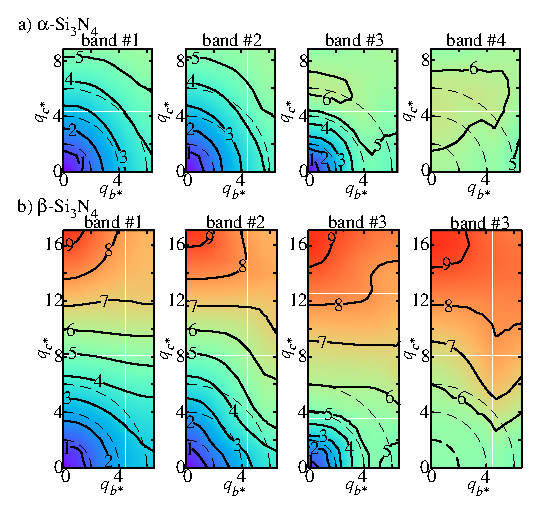
\includegraphics[width=\linewidth]{Fig2_small.eps} \caption{(color
  online) Contour maps of phonon frequency (THz) on the $b^*c^*$
  planes of Brillouin-zones. The coordination in the reciprocal plane 
   are in units of $10^{-2}$ \AA$^{-1}$. The maps for the four lowest-frequency
  phonon states are shown. The frequency landscapes are formed by simply
  connecting the frequencies of the same band indices, assigned by
  ascending order of frequency at the respective $\mathbf {q}$
  points. \label{fig:Fig3_338} }
 \centering
\end{figure}

We investigate the anisotropy in $\mathbf{v}_{\lambda}$ by using another geometry, that
is, a cross-section of the Brillouin-zone. Fig.~\ref{fig:Fig3_338} shows
counter maps of $\omega_{\lambda}$  on the $b^*c^*$ plane.  We show the
counter maps for the four lowest-frequency bands, because they
contribute significantly to the $\boldsymbol{\kappa}$.  There were no 
significant differences in the distributions between the $b^*c^*$ plane and the
other planes containing the $c^*$ axis.  Thus we select the $b^*c^*$ plane as a
representative.  In the $\alpha$ phase, the distributions of $\omega_{\lambda}$ are nearly
isotropic. Their gradients, the group velocities projected onto the plane, are
thus nearly isotropic. In the $\beta$ phase, the iso-frequency lines in $0.06
\le q_{c^*} \le 0.12$ \AA$^{-1}$ are rather parallel to the $q_{b^*}$ axis.
The $\mathbf{v}_{\lambda}$ in the $\beta$ phase orient closely to the
$c$ axis direction. This confirms the large anisotropy in $\mathbf{v}_{\lambda}$
of the acoustic and low-frequency optical branches in the $\beta$ phase.

\subsection{Frequency-dependences of $\boldsymbol{\kappa}^\text{c}$, $\mathbf{v}$$_\lambda$ and $\Gamma_\lambda$}

\begin{figure*}[ht]
 \begin{center}
  \includegraphics[width=0.9\linewidth]{figure_dos_jdos_kc_m1010.eps}
  \caption{(color online) Microscopic phonon properties of three Si$_3$N$_4$
	  phases. Cumulative thermal conductivity $\mathbf{\kappa}^\text{c}$ and its derivative
	  (a), DOS (b), weighted DOS with $v_{\lambda,i}^2$ (c) and linewidth $\Gamma_\lambda$ (d).
  \label{fig:Fig5_338_rev} }
 \end{center}
\end{figure*}

We have investigated in the previous two sections the anisotropy in
$\mathbf{v}_\lambda$, which gives an insight on the anisotropy in the
$\boldsymbol{\kappa}$. Here we completely investigate the characteristic points
in the $\boldsymbol{\kappa}$ by using the important phonon properties existing
in the closed form of RTA in Eq.~(\ref{eq:kappa}). These properties are taken
over the Brillouin zone, similar to $\boldsymbol{\kappa}$.
In order to investigate these properties with respect to the
phonon branches, we show in Fig.~\ref{fig:Fig5_338_rev} frequency
distributions of these properties: Phonon densities of states (DOS) in
Fig.~\ref{fig:Fig5_338_rev}-a show distributions of heat carriers. 
The first peak in DOS is denoted by an arrow. It is approximately associated
with flattening of acoustic branches near Brillouin zone boundaries.
Cumulative thermal conductivities $\boldsymbol{\kappa}^c$ 
show frequencies where phonons largely
contribute to $\boldsymbol{\kappa}$.  In Fig.~\ref{fig:Fig5_338_rev}-c,
$\boldsymbol{\kappa}^c$ and their
first derivatives are shown
in order to find the contributions clearly. We weighted the DOS with
\rm{v}$_{\lambda,i}^2$ and they are shown in Fig.~\ref{fig:Fig5_338_rev}-c. These
profiles show both of the impacts of \rm{v}$_{\lambda,i}$ and number of heat
carriers. We abbreviate these weighted DOS as WDOS. Phonon linewidths are a 
remaining important property.  They are shown as scatter plots $(\Gamma_\lambda,
\omega_\lambda)$ in Fig.~\ref{fig:Fig5_338_rev}-d. 

Among the panels in Fig.~\ref{fig:Fig5_338_rev}, the $\gamma$ phase has its DOS,
WDOS, and
$\Gamma_\lambda$ distribution much different from
the others, consistently with the large
differences in the crystal structure. Some of the remarkable differences are
explained by its characteristic chemical bonding: (1) In the DOS, the first peak is located at
a higher frequency than that of the other phases. This is consistent with the
finding in the band diagram; the linear dispersions of the acoustic phonon
branches with the large gradients. This reflects the strong chemical bonding as
indicated by the large bulk modulus. (2) In most of the frequencies with phonons
largely contributing to $\boldsymbol{\kappa}$, the $\gamma$ phase has WDOS 
next largest to the WDOS for $v_{\lambda,z}$ of the $\beta$ phase.
This is also explained by the large gradients in the acoustic phonon branches.
(3) In the same frequencies as mentioned in (2), the linewidths are larger than
those in the other phases. For this point, we investigate the
three-phonon-scattering strength $\Phi_{\lambda\lambda'\lambda''}$.  In
Table.~\ref{table:aveavepp}, the magnitudes of
$\Phi_{-\lambda\lambda'\lambda''}$ are compared as their averages over two
different
frequency ranges of $\omega_\lambda$ and all indices in $\lambda'$ and
$\lambda''$. Its average over $\omega_\lambda$ in 0--15 THz is much larger than
that of the other phases. This forms the larger linewidths.
Because of the opposite impacts of the linewidths and WDOS, the $\kappa^c_{xx}$
is relatively small. It resembles to the $\kappa^c_{xx}$ of the
$\beta$ phase.

\begin{table}[ht]
	\caption{\label{table:aveavepp} \textcolor{blue}{Averages of
	$\Phi_{-\lambda\lambda'\lambda''}$ over frequency ranges of
	$\omega_\lambda$ (0--15 and 0--35 THz) and all ($\lambda'$,$\lambda'$). The
	values are in units of 10$^{-10}$ eV$^2$f.u.$^{-1}$.}}
 \begin{ruledtabular}
  \begin{tabular}{cccc}
	  \multirow{2}{*}{Frequency Range (THz)}
   & \multicolumn{3}{c}{Phase}  \\
   \cline{2-4}
   & $\alpha$ & $\beta$ & $\gamma$ \\
   \hline
   \multirow{1}{*}{0--15}
   & \textcolor{blue}{2.66}  &  \textcolor{blue}{2.63}  & 5.76 &    
   \multirow{1}{*}{0--30}
   & \textcolor{blue}{13.1} & \textcolor{blue}{13.0} & 11.4 &     
  \end{tabular}
 \end{ruledtabular}
\end{table}

We hereafter compare the properties between the $\alpha$ and $\beta$ phases.
It is interesting that $\boldsymbol{\kappa}^c$ in the $\beta$ phase still
increase significantly in the higher frequency range than the DOS first peak
position.  In this frequency range, WDOS of the $\beta$ phase show still
large intensities.  The linewidths are distributed in a similar way for both of
the phases.  The DOS are similar as well.  Thus the significant increase in
$\boldsymbol{\kappa}^c$ across the DOS first peak position is ascribed only to the
large $\athbf{v}_\lambda$. The large $\mathbf{v}_\lambda$ in this frequency
range is consistent with the large dispersions of the branches in these
frequencies investigated in the previous sections. 
In Figs.~\ref{fig:Fig5_338_rev}-b and c, the profiles of
$\frac{d\boldsymbol{\kappa}^c_{ii}}{d\omega_\lambda}$ are characterized by those of WDOS
with $v_{\lambda,i}^2$ for the same directional indicies.  Because DOS and $\Gamma_{\lambda}$ are
similar between the phases, the anisotropy in $\mathbf{v}_\lambda$ simply accounts
for the different anisotropy in $\boldsymbol{\kappa}$  between the two
phases.  

It is still curious that $\Gamma_\lambda$ are similar between these phases
although $\mathbf{v}_\lambda$ have marked differences.  We investigate
this further.
As for not $\Gamma_{\lambda}$ but $\boldsymbol{\kappa}$, previously, Lindsay {\it et
al.}~\cite{Lindsay} found a significant positive correlation between the
$\boldsymbol{\kappa}$ and the number of the configurations for the three
phonons, $\{\lambda, \lambda', \lambda''\}$ (the phase space available for the
three-phonon scattering), among many crystals of the zincblende structure. 
Closely relateing to this, as for $\Gamma_{\lambda}$, $\Gamma_{\lambda}$
strongly depends on the number of configurations for the two phonons,
$\{\lambda', \lambda''\}$, available in the three-phonon scatering. This is
can be understood through the formula of $\Gamma_{\lambda}$ which  contains delta functions corresponding to the
selection rule of the three-phonon scattering~\cite{phono3py}. 
A distribution of the configurations is represented
as a joint density of states (JDOS), ${D_2(\mathbf{q},\omega)}$,  
\begin{align}
 \label{eq:jdos}
 &D_2(\mathbf{q},\omega) = D_2^{(1)}(\mathbf{q},\omega) +  D_2^{(2)}(\mathbf{q},\omega)
\end{align}
where 
\begin{eqnarray*}
	D_2^{(1)} & = & \frac{1}{N} \sum_{\lambda'\lambda''}\Delta(-\mathbf{q} + \mathbf{q'} + \mathbf{q''}) \nonumber \\
								   & \times & [\delta(\omega + \omega_{\lambda'} - \omega_{\lambda''}) + \delta(\omega - \omega_{\lambda'} + \omega_{\lambda''})],\\
	D_2^{(2)} & = & \frac{1}{N} \sum_{\lambda'\lambda''}\Delta(-\mathbf{q} + \mathbf{q'} + \mathbf{q''}) \nonumber \\
								   & \times & \delta(\omega - \omega_{\lambda'} - \omega_{\lambda''}),
\end{eqnarray*}
with $\Delta$($\mathbf{x}$) giving 1 if $\mathbf{x}$ is a reciprocal lattice
vector and otherwise zero.  JDOS were employed to analyze the linewidths
$\Gamma_{\lambda}$ of Ge$_2$Sb$_2$Te$_5$~\cite{mukhopadhyay-ltc} and the
imaginary parts of the self energy $\Gamma_{\lambda}(\omega)$ of many
zincblende and wultzite polymorphs~\cite{phono3py}.  Following to these studies,
we employ the JDOS to examine the similarity between $\Gamma_{\lambda}$ 
of the $\alpha$ and $\beta$ phases.

Fig.~\ref{fig:Fig6_338} shows the frequency-functions of JDOS at different
$\mathbf{q}$-points on the $\Gamma$--A and $\Gamma$-K paths. There are very
weak $\mathbf{q}$-point dependences among the functions.  At the low frequency
region with phonons largely contributing to the $\boldsymbol{\kappa}$, among the two terms of
$D_2^{(1)}$ and $D_2^{(2)}$ in Eq.~(\ref{eq:jdos}), dominant is
$D_2^{(2)}$.
The $D_2^{(2)}$ basically corresponds to the half part ($\omega \geq  0$) of the
auto-correlation function of the DOS. The DOS for both of the $\alpha$ and $\beta$
phases show the frequency gap (Fig.~\ref{fig:Fig5_338_rev}-a). The $D_2^{(2)}$
reflect this DOS feature, dropping suddenly around 0 THz and showing a
small shoulder around 5 THz, which corresponds to the width of the gap. Moreover
the $D_2^{(2)}$ shows a broad peak around 18 THz, which corresponds to the frequency
shift to make the largest correlation between the higher and lower portions of
DOS across the gap.  Because the gap is  originated from the
differences in the vibrations of the planer NSi$_3$ contained in both of the
$\alpha$ and $\beta$ crystal structures,~\cite{kuwabara} the major shapes of the $D_2^{(2)}$,
reflecting this gap feature, are similar in these phases. With the same origin,
the $D_2^{(1)}$ are also similar in these phases. 
As indicated in Table.~\ref{table:aveavepp}, the $\Phi_{-\lambda\lambda'\lambda''}$
have similar impacts on the linewidths. 
With these similar impacts of
the JDOS and $\Phi_{-\lambda\lambda'\lambda''}$,
$\Gamma_\lambda$ in Fig.~\ref{fig:Fig5_338_rev}-d are similar.  

\begin{figure}[ht]
 \centering
  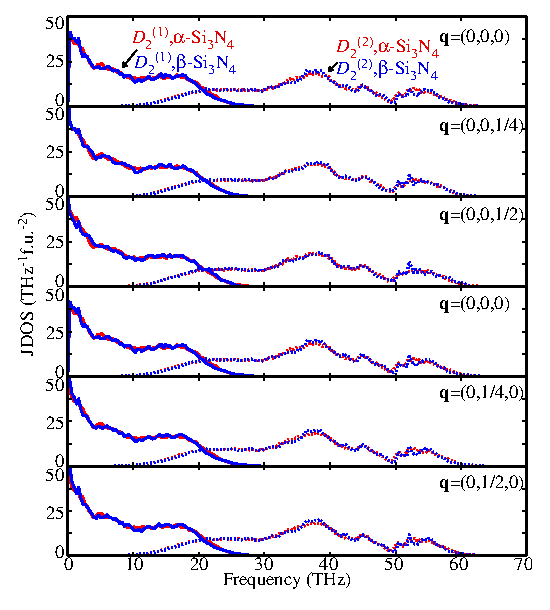
\includegraphics[width=0.9\linewidth]{figure_jdoss.eps} \caption{(color
	  online) \textcolor{blue}{JDOS of $\alpha$- and $\gamma$-Si$_3$N$_4$ at different $\mathbf q$ points.
  The first and forth rows are JDOS at the same $\Gamma$-point but calculated with the polarization for non-analytic term correction set along $c^*$ and $b^*$, respectively.} \label{fig:Fig6_338} }
 \centering
\end{figure}

As a small but interesting difference in linewidths distributions, 
$\Gamma_\lambda$ below 5 THz are aligned on a
single smooth line in the $\alpha$ phase, while those in the $\beta$ phase are
scattered roughly on two lines. This difference is investigated with 
directions of the atomic vibrations of the phonons. In Fig.~\ref{fig:Fig7_338}-a, the $\Gamma_\lambda$ are
classified using colors according to the sums of the squares of the eigenvector
components along the $\mathbf{q}$; the sum is 1 for a perfectly longitudinal
wave. However, these sums have no clear contrast to distinguish the two branches
in the $\beta$ phase.  Fig.~\ref{fig:Fig7_338}-b shows the same plot as
Fig.~\ref{fig:Fig7_338}-a, but with colors according to the sums of the squares
of the eigenvector components along the $ab$ plane, which has 1 when the
eigenvectors lie on the $ab$ plane. There is a tendency in the $\beta$ phase
that  $\Gamma_\lambda$ are large for vibrations along the $ab$ plane.
Therefore, within the single-mode RTA, for the phonon modes below 5 THz, all of
which belong to the acoustic phonon branches, vibration modes along the $ab$
plane are more easily scattered in the $\beta$ phase, no matter whether they are
longitudinal or transverse. For the panel of $\beta$-Si$_3$N$_4$ in
Fig.~\ref{fig:Fig7_338}-b, a straight line can divide the phonon modes into the
two groups. The numbers of the phonon modes in the upper and lower parts are 157
and 58, whose ratio is consistent to the population ratio of the vibration modes
along and out of the $ab$ plane.


\begin{figure}[ht]
 \centering
  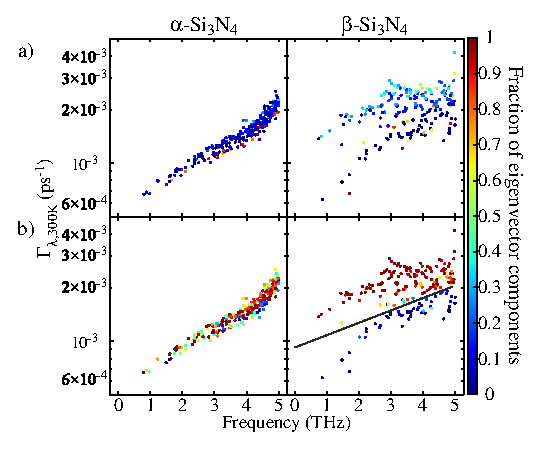
\includegraphics[width=\linewidth]{figure_analyze_gamma3_m1010_print.eps} \caption{(color
	  online) \textcolor{blue}{Distribution of linewidths $\omega_\lambda$ $\leq$ 5 THz
		  with colormaps with respect to strengths of eigenvector components along $\mathbf q$ (a)
		  and on $a$-$b$ plane (b).} \label{fig:Fig7_338}} 
 \centering
\end{figure}

% gv weighted dos
%\begin{align}
% \label{eq:v2dos}
% \langle\text{v}^2_i(\omega)\rangle = \frac{1}{N_\mathbf{q}\Omega}
% \int_0^\omega \sum_\lambda
% \text{v}_{\lambda,i}^2\delta(\omega'-\omega)d\omega'.
%\end{align}

\section{Summary}

In the present study, we investigate the lattice thermal conductivities of the
three Si$_3$N$_4$ phases, by using the lattice dynamics based on the {\it
ab-initio} interatomic force constants. The main remarks are as follows:

1) In the $\alpha$- and $\beta$-Si$_3$N$_4$, whose crystal structures are
characterized by the stacking manners of the basal layer structures, which
largely alter $\boldsymbol{\kappa}$. In $\alpha$-Si$_3$N$_4$, the
$\boldsymbol{\kappa}$ are rather isotropic, while the $\kappa$$_{zz}$ in the
$\beta$ phase is much larger than the $\kappa$$_{xx}$, showing remarkable
anisotropy in the $\boldsymbol{\kappa}$. The $\kappa_{xx}$ in the $\beta$ phase
is 2 times or more larger than the others $\kappa_{ii}$ in the three phases.

2) In the $\alpha$ phase, the acoustic mode phonons below 6 THz are the main
heat carriers, while in the $\beta$ phase, the phonons below 12 THz contribute
to the $\boldsymbol{\kappa}$. The group velocities alone qualitatively explains
this and the different anisotropy in $\boldsymbol{\kappa}$ between the $\alpha$
and $\beta$ phases.

3) In the $\gamma$ phase, the $\kappa_{xx}$ is relatively small. The
$\kappa^c_{xx}$ is similar to that of $\beta$-Si$_3$N$_4$.  Its number of heat
carriers, group
velocities and linewidths are much different from those of the other phases.
They are not set toward high $\kappa_{xx}$.

\section*{ACKNOWLEDGMENTS}
The present work was partly supported by Grants-in-Aid for Scientific
Research of MEXT, Japan (Grant No. 15K14108 and ESISM (Elements Strategy
Initiative for Structural Materials) of Kyoto University).

\appendix
\section{Pressure dependence of LTC of $\gamma$-phase}
\begin{figure}[ht]
 \begin{center}
  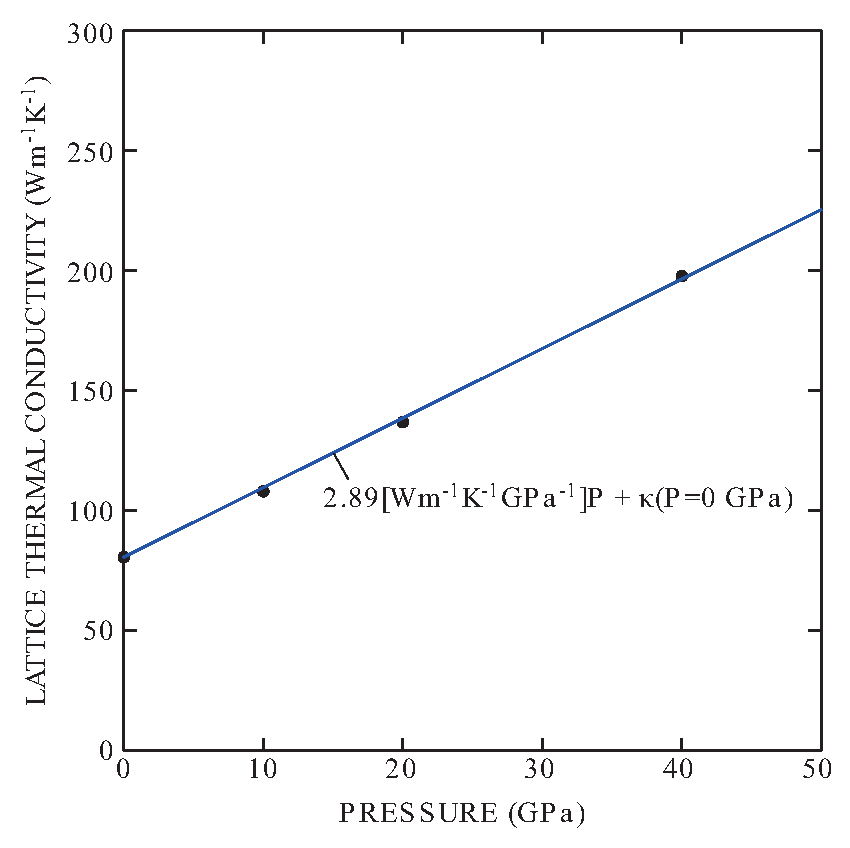
\includegraphics[width=0.80\linewidth]{S1.eps} \caption{(color online)
  Pressure dependence of LTC of $\gamma$-Si$_3$N$_4$.  \label{fig:S1} }
 \end{center}
\end{figure}
\bibliography{Si3N4}
\end{document}
